%%%%%%%%%%%%%%%%%%%%%%%%%%%%%%%%%%%%%%%%%%%%%%%%%%%%%%%%%%%%
%%  This Beamer template was created by Cameron Bracken.
%%  Anyone can freely use or modify it for any purpose
%%  without attribution.
%%
%%  Last Modified: January 9, 2009
%%

\documentclass[xcolor=x11names,compress, graphics]{beamer}

%% General document %%%%%%%%%%%%%%%%%%%%%%%%%%%%%%%%%%
\usepackage{graphicx}
\usepackage{tikz}
\usetikzlibrary{decorations.fractals}
%%%%%%%%%%%%%%%%%%%%%%%%%%%%%%%%%%%%%%%%%%%%%%%%%%%%%%
\usepackage{movie15}
\usepackage{float}
\usepackage{subfig}
\usepackage{amsmath}
\usepackage{amsfonts}
\usepackage{mathrsfs}
\usepackage{mathtools}

\usepackage{algorithm, algorithmic}

%% Beamer Layout %%%%%%%%%%%%%%%%%%%%%%%%%%%%%%%%%%
\useoutertheme[subsection=false,shadow]{miniframes}
\useinnertheme{default}
\usefonttheme{serif}
\usepackage{palatino}

\setbeamerfont{title like}{shape=\scshape}
\setbeamerfont{frametitle}{shape=\scshape}

\setbeamercolor*{lower separation line head}{bg=DeepSkyBlue4} 
\setbeamercolor*{normal text}{fg=black,bg=white} 
\setbeamercolor*{alerted text}{fg=red} 
\setbeamercolor*{example text}{fg=black} 
\setbeamercolor*{structure}{fg=black} 
 
\setbeamercolor*{palette tertiary}{fg=black,bg=black!10} 
\setbeamercolor*{palette secondary}{fg=black,bg=black!10}
\setbeamercolor*{palette quaternary}{fg=black,bg=black!10} 

%% Set the background and font color of the blocks 
\setbeamercolor{block title}{bg=DeepSkyBlue4,fg=white}

%% Set the type of the blocks
\setbeamertemplate{blocks}[shadow=true]

\newcommand{\topline}{%
  \tikz[remember picture,overlay] {%
    \draw[DeepSkyBlue4] ([yshift=-1.5cm, xshift = 1cm]current page.north west)
             -- ([yshift=-1.5cm,xshift=\paperwidth-1cm]current page.north west);}}
             
\setbeamertemplate{section in toc}[sections numbered]           

\renewcommand{\(}{\begin{columns}}
\renewcommand{\)}{\end{columns}}
\newcommand{\<}[1]{\begin{column}{#1}}
\renewcommand{\>}{\end{column}}

\usepackage[skip=10pt,font=scriptsize]{caption}
\captionsetup[figure]{labelformat=empty}

\DeclarePairedDelimiter\floor{\lfloor}{\rfloor}

\makeatother
\setbeamertemplate{footline}
{
  \leavevmode%
  \hbox{%
  \begin{beamercolorbox}[wd=.4\paperwidth,ht=2.25ex,dp=1ex,center]{author in head/foot}%
    \usebeamerfont{author in head/foot}\insertshortauthor
  \end{beamercolorbox}%
  \begin{beamercolorbox}[wd=.6\paperwidth,ht=2.25ex,dp=1ex,center]{title in head/foot}%
    \usebeamerfont{title in head/foot}\insertshorttitle\hspace*{3em}
    \insertframenumber{} / \inserttotalframenumber\hspace*{1ex}
  \end{beamercolorbox}}%
  \vskip0pt%
}
\makeatletter
%%%%%%%%%%%%%%%%%%%%%%%%%%%%%%%%%%%%%%%%%%%%%%%%%%

\title{\scshape \textbf{Divide And Conquer Paradigm}}
\author{\scriptsize\scshape Angel No\'e Mart\'inez Gonz\'alez}


\begin{document}

% The title page
\begin{frame}
\setcounter{framenumber}{1}
\titlepage
\scriptsize

\end{frame}
%===============


\section[\scshape Paradigm]{\scshape Paradigm}
\begin{frame}[allowframebreaks]{The Paradigm}
\topline

Solves a problem \textbf{recursively} applying at each level of the recursion

\begin{itemize}
	\item {\scshape\textbf{DIVIDE}} the problem into smaller sub-problems.
	\item {\scshape\textbf{CONQUER}} via recursive calls.
	\item {\scshape\textbf{COMBINE}} solutions of sub-problems into one for the original problem.
\end{itemize}

Also consider a \textbf{base case} when the sub-problems become small enough.


\framebreak
\topline

{\scshape\Large Merge Sort: Retaken}

\begin{minipage}{5cm}

\captionof*{algorithm}{}{{\scshape merge-sort}($A, p, r$)}
\begin{algorithmic}[1]
\IF{$p<r$}
	\STATE $q = \floor*{(p+r)/2}$
	\STATE {\scshape merge-sort}($A, p, q$)
	\STATE {\scshape merge-sort}($A, q, r$)
	\STATE {\scshape merge}($A, p, q, r$)
\ENDIF
\end{algorithmic}

\end{minipage}\ \ 
\begin{minipage}{5cm}

\captionof*{algorithm}{}{{\scshape merge}($A, p, q, r$)}
\begin{algorithmic}[1]
\STATE $B=1^{st}$ part of array.
\STATE $C=2^{nd}$ part of array.
\STATE $i=1,j=1$
\FOR{$k=1$ to $n$}
	\IF{$B[i]<C[j]$}
		\STATE $A[k]=B[i++]$
	\ELSE
		\STATE $A[k]=C[j++]$
	\ENDIF
\ENDFOR
\end{algorithmic}
\end{minipage}


\framebreak
\topline

{\scshape\Large Insights}

\begin{itemize}
	\item Sub-problems sizes can be any! e.g. $1/2$, $1/3$, etc.
	\item Base case is often too naive.
	\item Generally, in the third step relies the good performance.
	\item Trying to make third step simple is the best way to tackle the problem.
\end{itemize}


\end{frame}


\section[\scshape Recurrences]{\scshape Recurrences}
\begin{frame}[allowframebreaks]{Recurrences}
\topline

{\scshape\Large A Recurrence}
\begin{itemize}
	\item provide a natural way to describe the running time of divide-and-conquer algorithms.
	\item describes $T(n)$ in terms of the running time of recursive calls.
	\item consider a base case for which

	$$
	T(n) \leq a
	$$	
	
	\item consider the larger imputs as
	
	$$
	T(n) \leq f(n)
	$$
	
\end{itemize}

%Recall $T(n)$ is the number of operation an algorithm requires to solve a problem.

\framebreak
\topline

{\scshape Computing Recurrences: Merge Sort}

\begin{itemize}
	\item Base case: sort two numbers. Swap positions in the worst case.

	$$
	T(1) = 1
	$$	
	
	\item Larger inputs: two sub-problems of size $n/2$ plus one call to merge with size $n$, i.e.
	
	$$
	T(n)=2T(n/2) + \Theta(n)
	$$
	
\end{itemize}

\framebreak
\topline

leading to

$$
T(n) =
\begin{cases}
\Theta(1) & \text{if $n=1$}\\
2T(n/2) + \Theta(n) & \text{if $n>1$}
\end{cases}
$$

help us to get the running time

$$
T(n) = \Theta(n\log_2 n)
$$

and for the properties of asymptotic notation $T(n) = O(n\log n)$

\end{frame}


\section[\scshape Counting Inversions]{\scshape Counting Inversions}
\begin{frame}[allowframebreaks]{Example: Counting Inversions}
\topline

{\scshape\Large Motivation}

\begin{itemize}
	\item List of ranked objects $A=[a_1,a_2,a_3,...,a_n]$ and a reference list $B$.
	\item We want to figure out how similar these lists are.
	\item Application {\color{blue}Collaborative Filtering}.
\end{itemize}

Let $B$ be the sorted list of $A$, then what we seek is the number of inversions in list $A$, i.e. the number of pairs $(i,j)$ such that

$$
i<j \text{\ and \ } A[i] > A[j]
$$

\framebreak
\topline

{\scshape\Large Example: $A=[1,3,5,2,4,6]$}\\
\vspace{0.5cm}
\begin{minipage}{3cm}
Inversions:

$$
(3,2), (5,2), (5,4)
$$

\end{minipage}\ \ 
\begin{minipage}{7cm}

\begin{figure}
	\begin{center}
		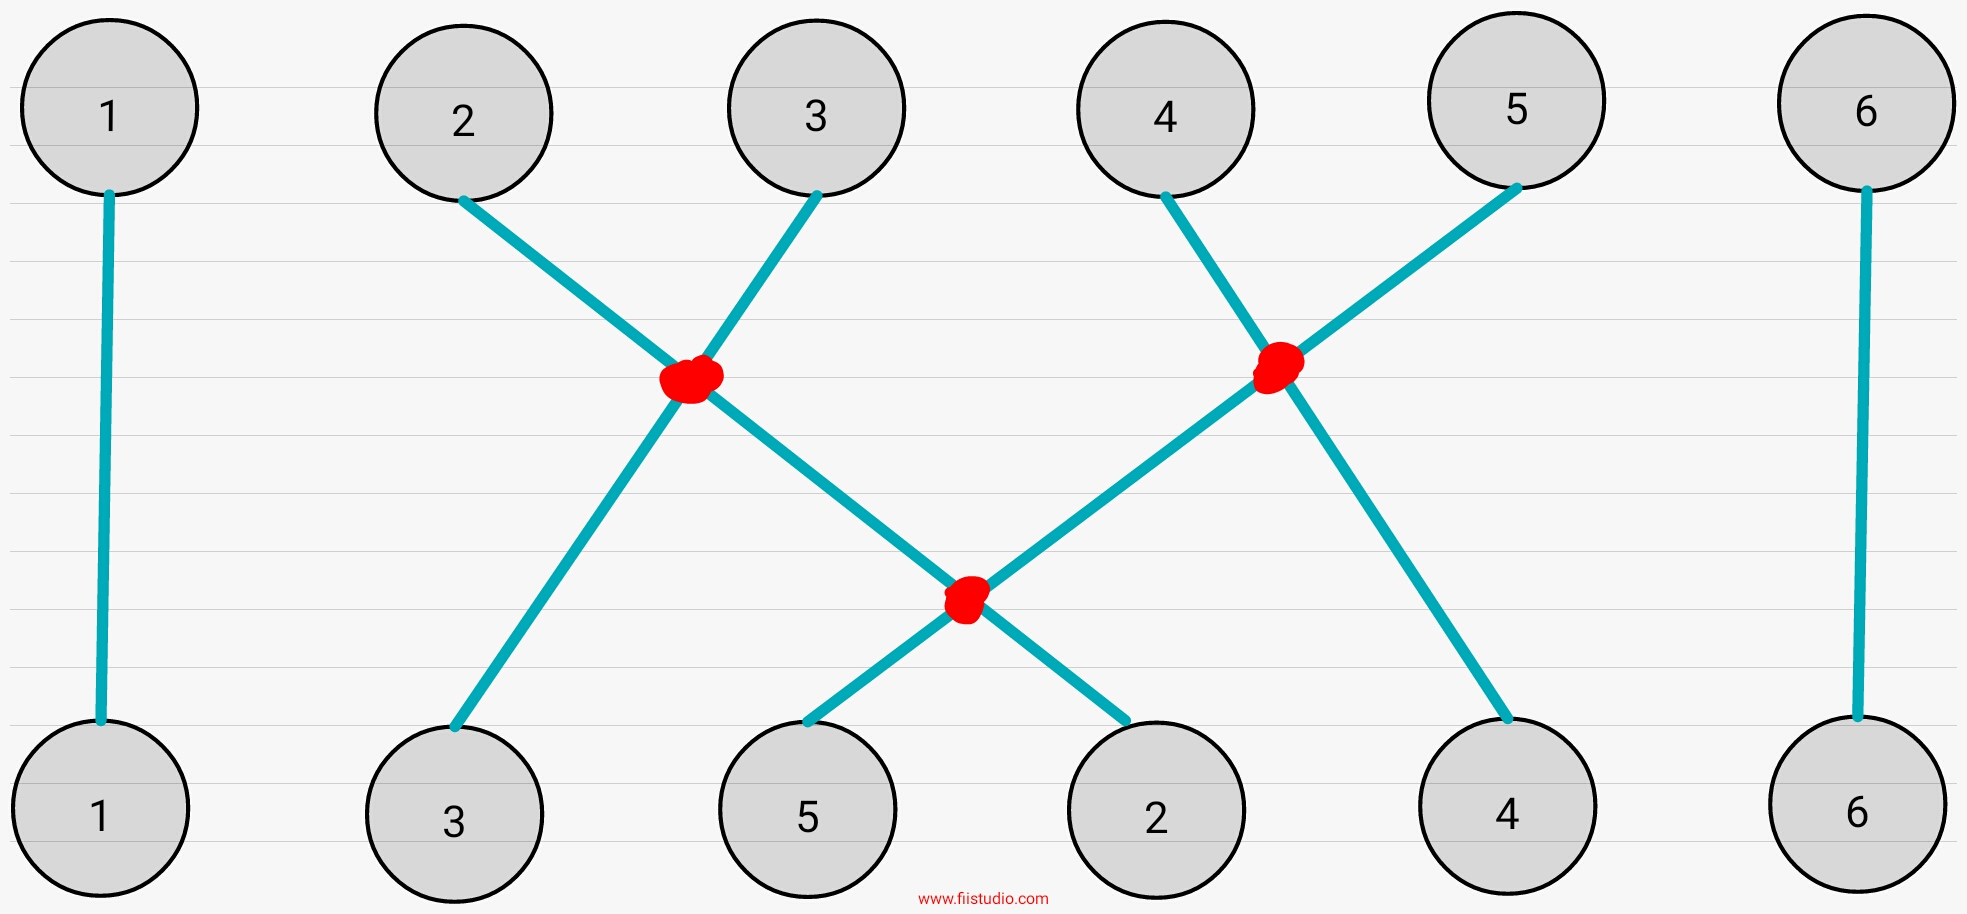
\includegraphics[width=8cm]{Figures/inversions.jpg}
	\end{center}
\end{figure}

\end{minipage}\\
\vspace{.5cm}
{\small In general the upper bound of number of inversions is $n(n-1)/2$.}


\framebreak
\topline

A brute force algorithm

\begin{minipage}{5cm}
\captionof*{algorithm}{}{{\scshape Brute-Force}($A, n$)}
\begin{algorithmic}[1]
\STATE $count = 0$
\FOR{$i=1,...,n$}
	\FOR{$j=i+1,...,n$}
		\IF{$A[i]>A[j]$}
			\STATE $count = count +1 $
		\ENDIF
	\ENDFOR
\ENDFOR
\RETURN count
\end{algorithmic}
\end{minipage}\ \ \ \ 
\begin{minipage}{5cm}

It is correct but

$$
T(n) = O(n^2)
$$

We can do better!

\end{minipage}


\framebreak
\topline

The key idea is to use divide and conquer. Let be $(i,j)$ an inversion with $i<j$

\begin{enumerate}
	\item Let's call it a left inversion if $i,j \leq n/2$.
	\item Let's call it a right inversion if $i,j > n/2$.
	\item Let's call it a split inversion if $i \leq n/2 < j$
\end{enumerate}

compute 1 and 2 recursively and implement other routine for 3.

\framebreak
\topline

{\large
\captionof*{algorithm}{}{{\scshape Count-Inversions}($A, n$)}
\begin{algorithmic}[1]
\IF{$n=1$}
	\RETURN $0$
\ENDIF
\STATE $x$={\scshape Count-Inversions}(first half of $A$, $n/2$)
\STATE $y$={\scshape Count-Inversions}(second half of$A$, $n/2$)
\STATE $z$={\scshape Count-Split-Inversions}($A, n/2$)
\RETURN $x+y+z$
\end{algorithmic}
}
\vspace{0.5cm}
The goal is to implement efficiently {\scshape Count-Split-Inversions} for good performance.

\framebreak
\topline

The key idea to implement {\scshape Count-Split-Inversions} is to consider sorting, more precisely the merge sub-routine of merge-sort

\begin{minipage}{5cm}
\begin{itemize}
	\item $B=$ left part of array.
	\item $C=$ second part of array.
	\item $A=$ output array.
\end{itemize}

\end{minipage}\ \ 
\begin{minipage}{5cm}

\captionof*{algorithm}{}{{\scshape merge}($A, p, q, r$)}
\begin{algorithmic}[1]
\STATE $i=1,j=1$
\FOR{$k=1$ to $n$}
	\IF{$B[i]<C[j]$}
		\STATE $A[k]=B[i++]$
	\ELSE
		\STATE $A[k]=C[j++]$
	\ENDIF
\ENDFOR
\end{algorithmic}
\end{minipage}


\framebreak
\topline

Now suppose $A$ has no split inversions, then following properties holds

\begin{itemize}
	\item All elements in $B$ are less than the elements in $C$.
	\item All elements in $B$ are copied back to $A$ before the elements in $C$.
\end{itemize}


The second half has the clue to discover the inversions!

\framebreak
\topline

\begin{figure}
	\begin{center}
		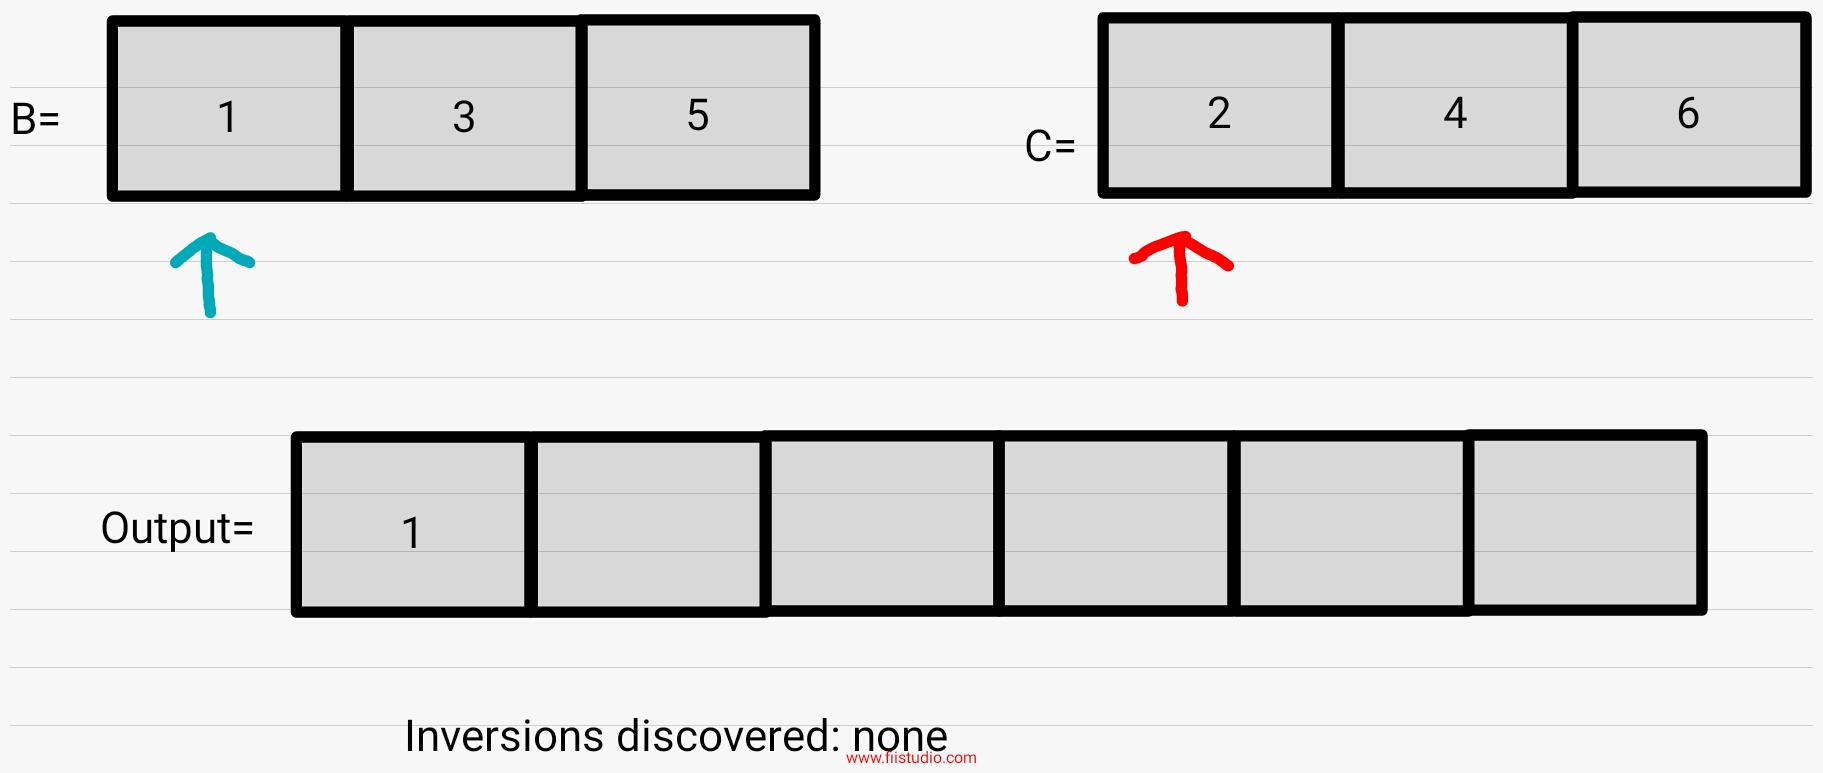
\includegraphics[width=10cm]{Figures/inv1.jpg}
	\end{center}
\end{figure}

\framebreak
\topline

\begin{figure}
	\begin{center}
		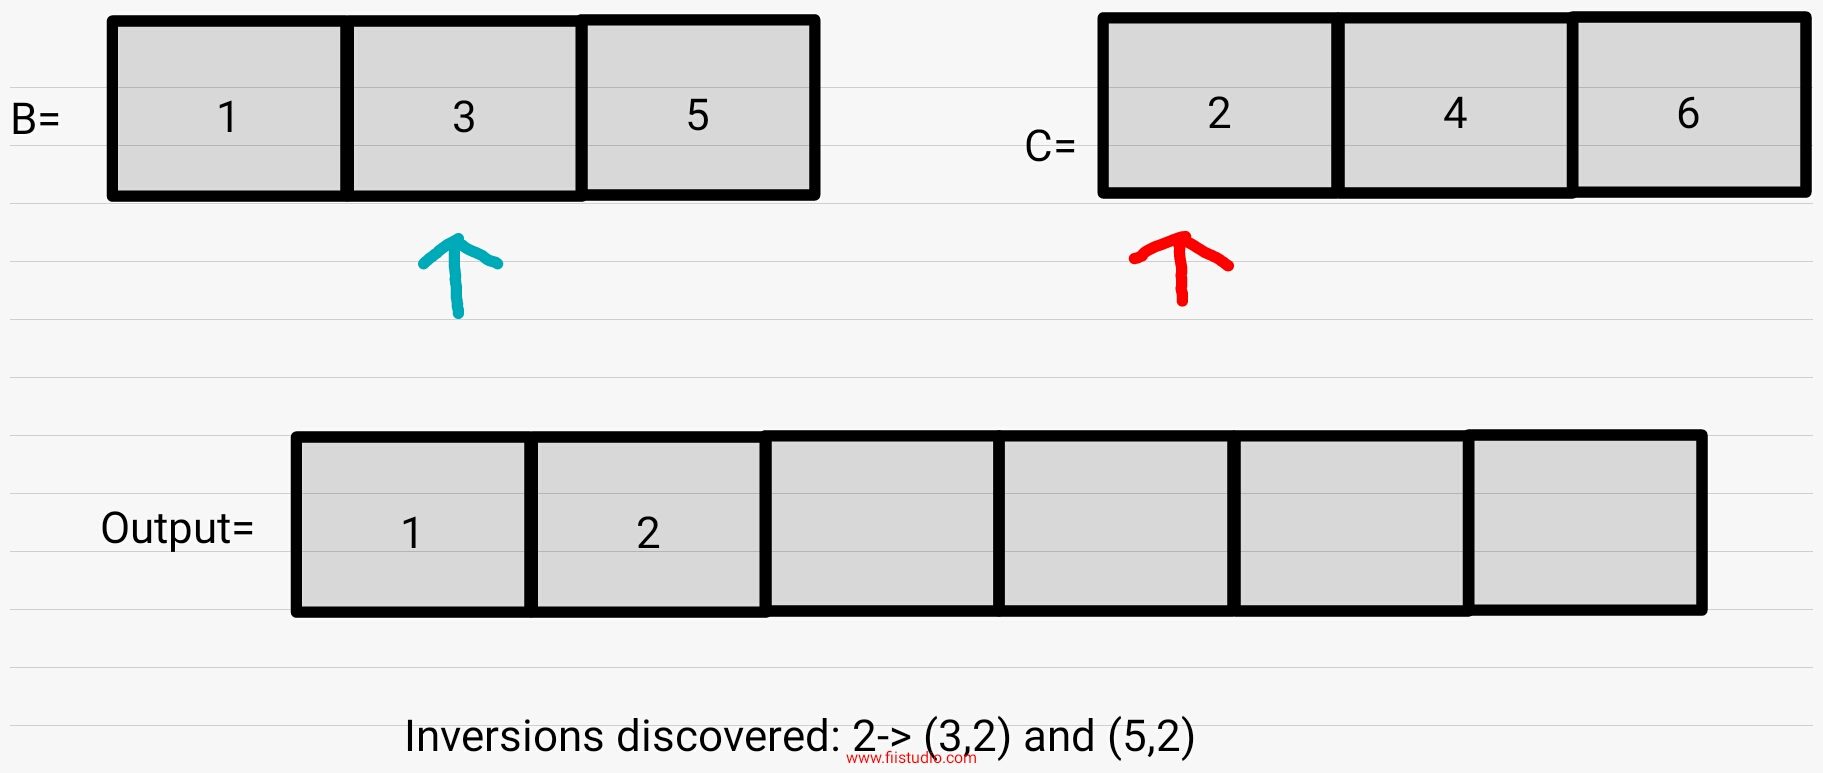
\includegraphics[width=10cm]{Figures/inv2.jpg}
	\end{center}
\end{figure}


\framebreak
\topline

\begin{figure}
	\begin{center}
		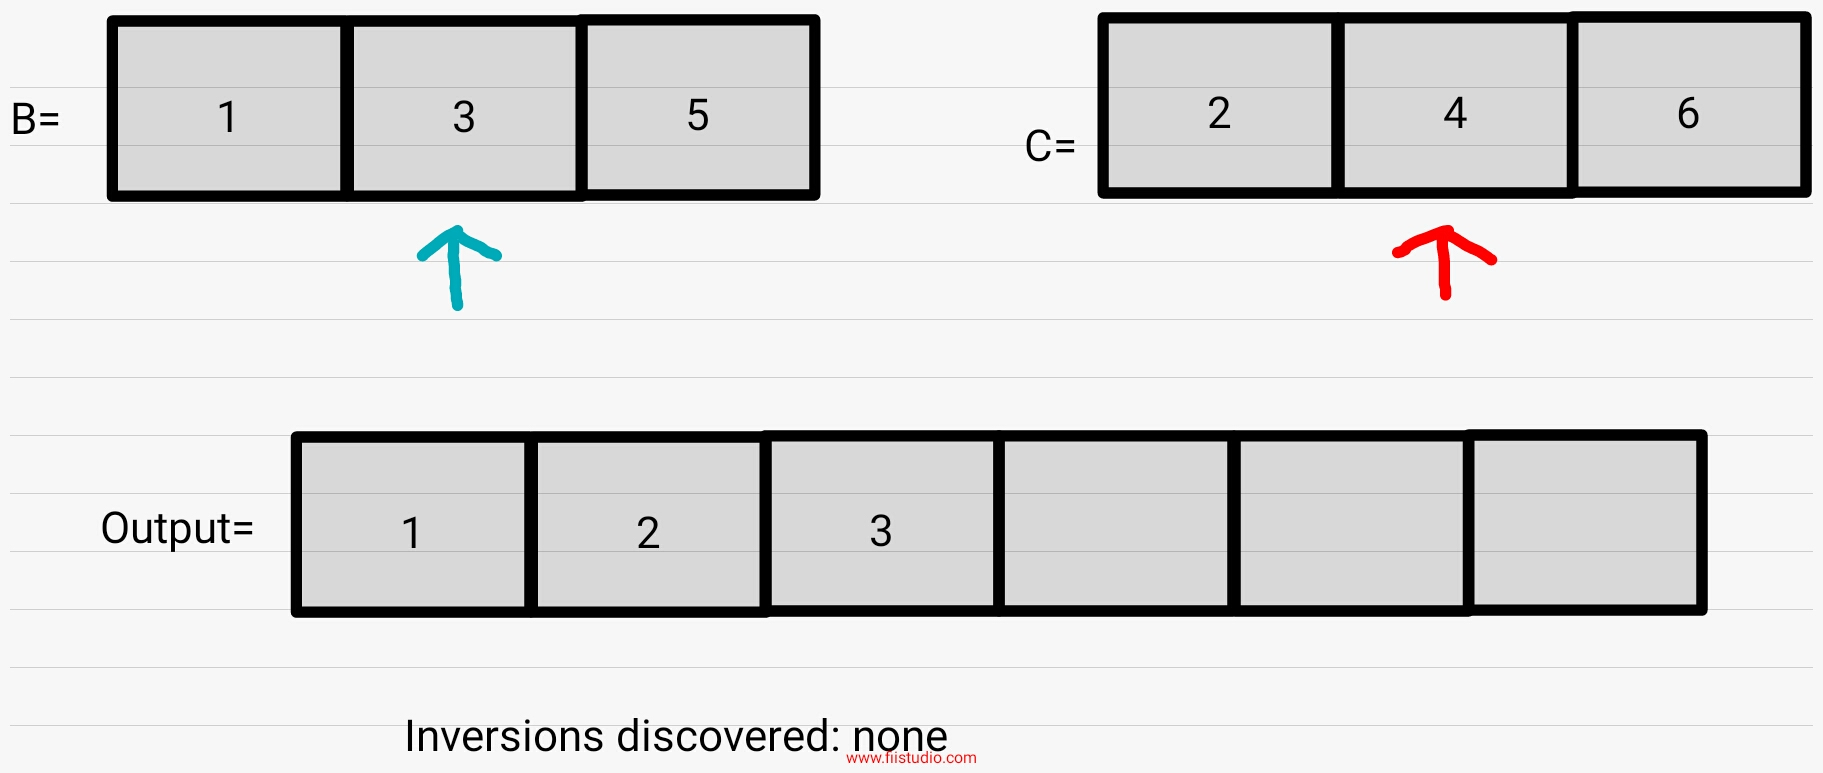
\includegraphics[width=10cm]{Figures/inv3.jpg}
	\end{center}
\end{figure}


\framebreak
\topline

\begin{figure}
	\begin{center}
		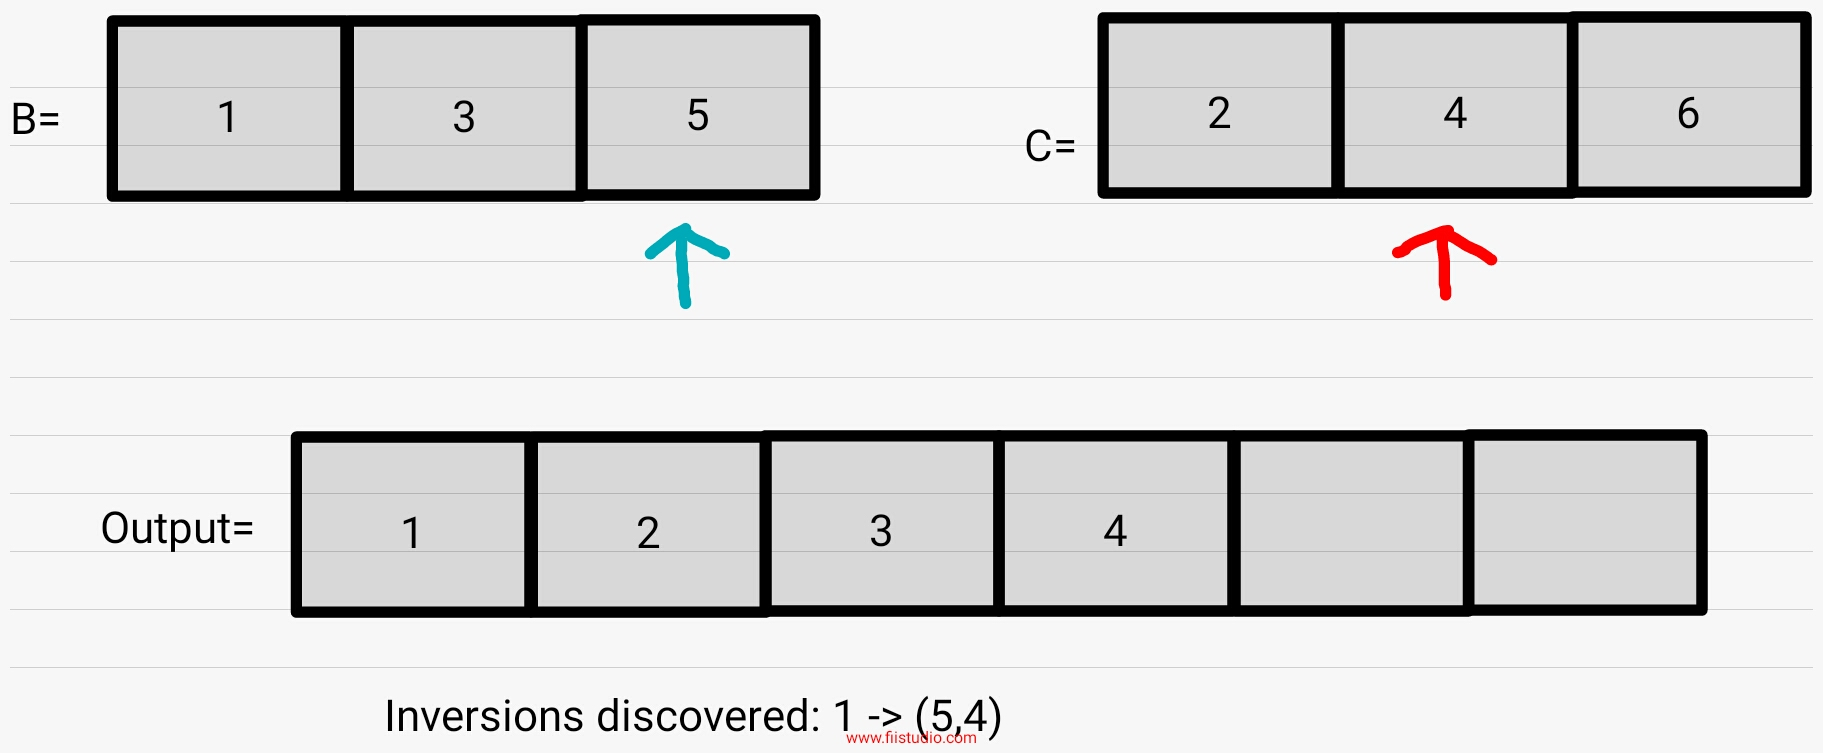
\includegraphics[width=10cm]{Figures/inv4.jpg}
	\end{center}
\end{figure}

\framebreak
\topline

\begin{figure}
	\begin{center}
		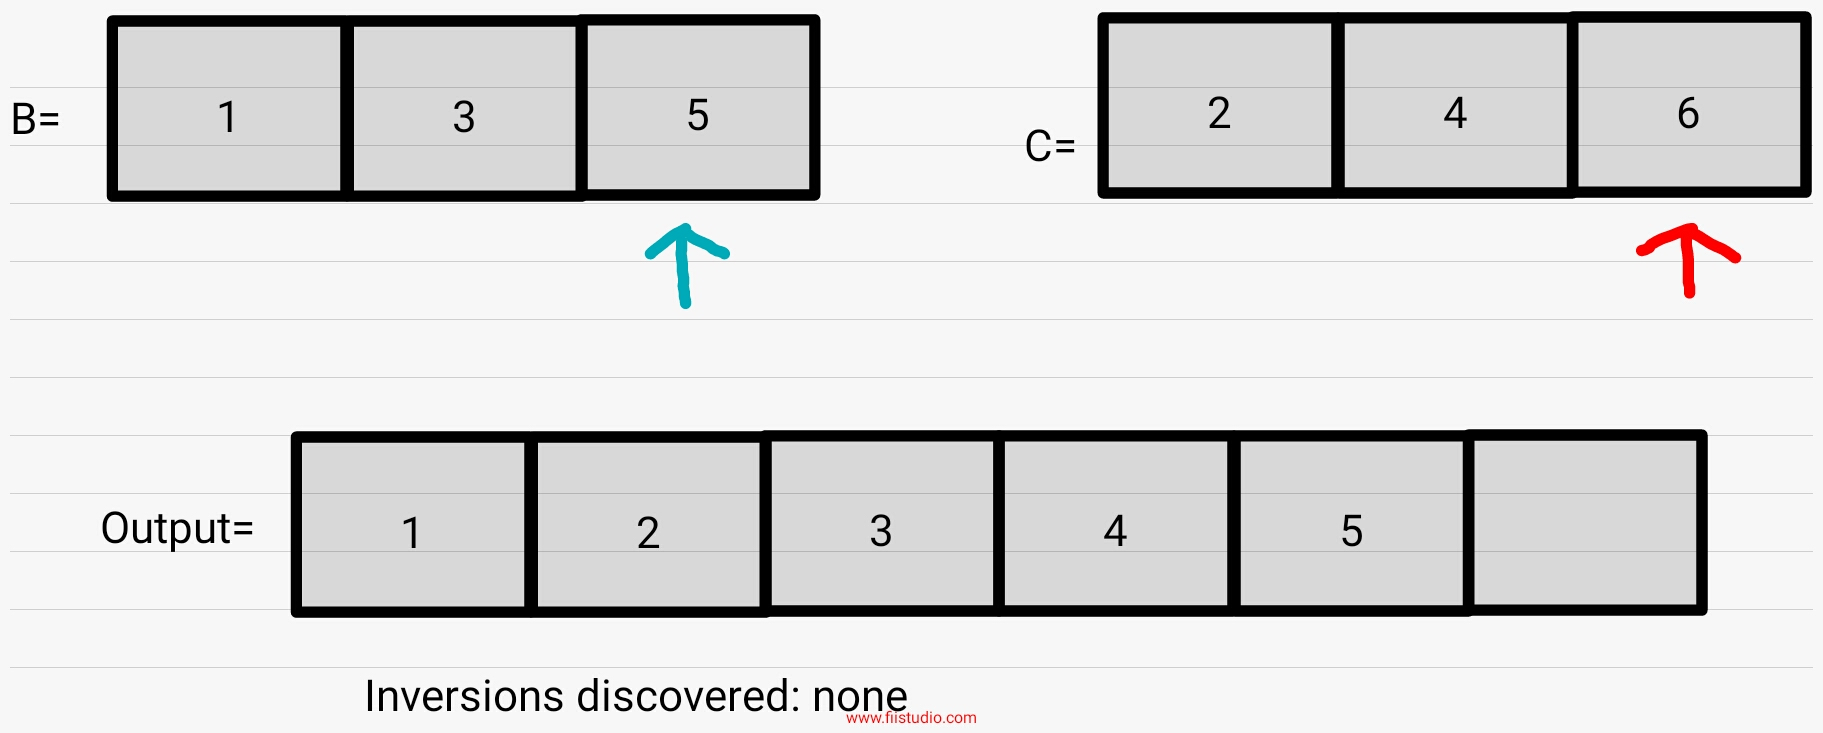
\includegraphics[width=10cm]{Figures/inv5.jpg}
	\end{center}
\end{figure}

\framebreak
\topline

\begin{figure}
	\begin{center}
		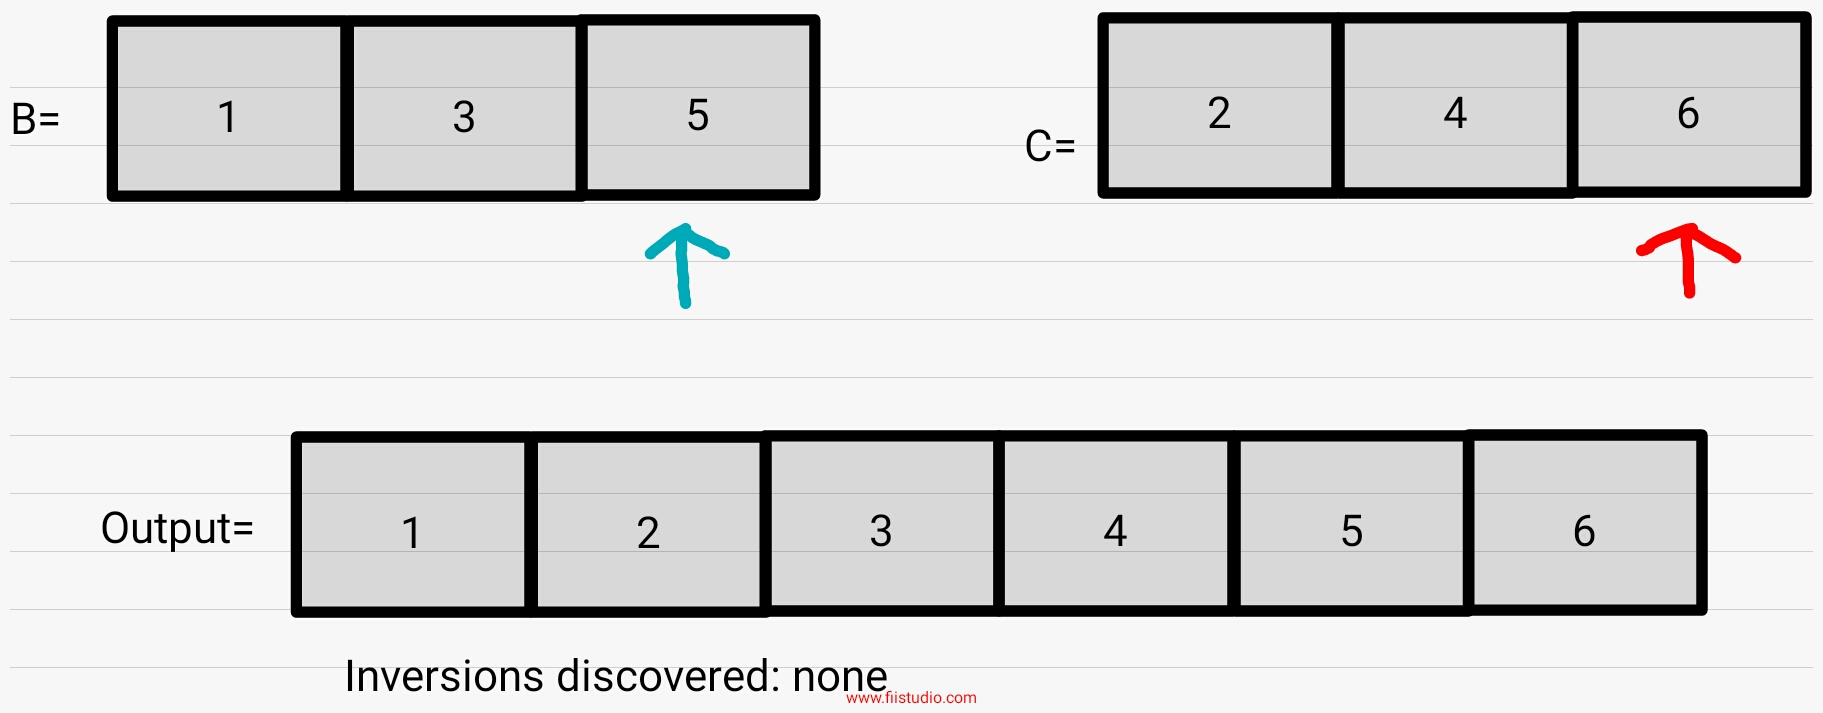
\includegraphics[width=10cm]{Figures/inv6.jpg}
	\end{center}
\end{figure}

\framebreak
\topline

The split inversions involving an element $y_i\in C$ is the number of remaining positions from $i$ in $B$ when it is copied to the output array $D$.

\begin{figure}
	\begin{center}
		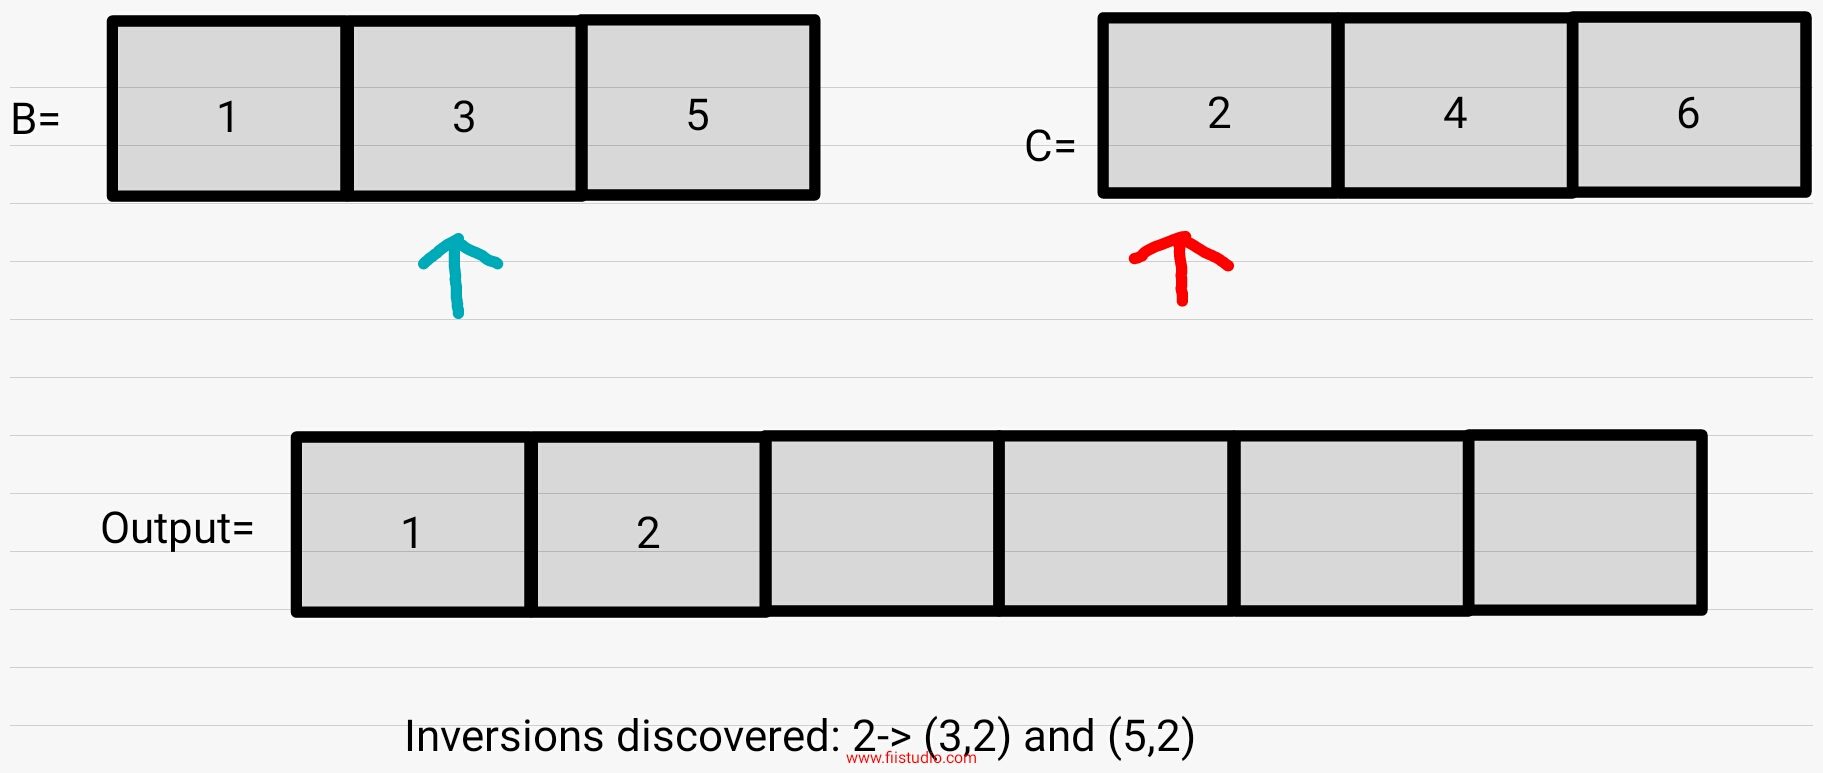
\includegraphics[width=10cm]{Figures/inv2.jpg}
	\end{center}
\end{figure}


\framebreak
\topline

{\scshape\Large The Algorithm}

{\large
\captionof*{algorithm}{}{{\scshape Count-Inversions}($A, n$)}
\begin{algorithmic}[1]
\IF{$n=1$}
	\RETURN $0$
\ENDIF
\STATE $B,x$={\scshape Count-Inversions}(first half of $A$, $n/2$)
\STATE $C,y$={\scshape Count-Inversions}(second half of$A$, $n/2$)
\STATE $D,z$={\scshape Count-Split-Inversions}($B, C, n/2$)
\RETURN $x+y+z, D$
\end{algorithmic}
}

\framebreak
\topline
\begin{minipage}{5cm}
\captionof*{algorithm}{}{\scriptsize{\scshape Count-Split-Inversions}($B, C, n$)}
\begin{algorithmic}[1]
\STATE $i=1,j=1$,$inv=0$
\FOR{$k=1$ to $n$}
	\IF{$B[i]<C[j]$}
		\STATE $D[k]=B[i++]$
	\ELSE
		\STATE $inv+=n/2-i$
		\STATE $D[k]=C[j++]$
	\ENDIF
\ENDFOR
\RETURN $inv, D$
\end{algorithmic}
\end{minipage}\ \ \ 
\begin{minipage}{5cm}

The recurrence is

$$
T(n) =
\begin{cases}
O(1) & \text{if $n=1$}\\
2T(n/2) + O(n) & \text{if $n>1$}
\end{cases}
$$

What is the running time?

\end{minipage}


\end{frame}


\section[\scshape Solving Recurrences]{\scshape Solving Recurrences}
\begin{frame}{Solving Recurrences : Recursion Tree}
\topline

\begin{figure}
	\begin{center}
		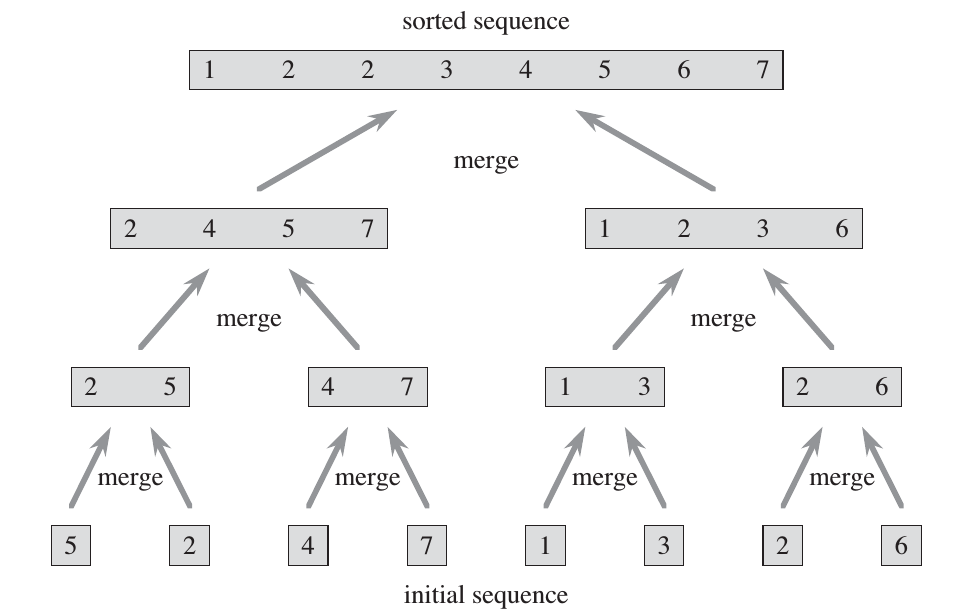
\includegraphics[width=8cm]{Figures/mergeSortTree.png}
	\end{center}
\end{figure}

At each level $j=0,1,...,log_2(n)$, there are $2^j$ subproblems of size $n/2^j$.

\end{frame}

\begin{frame}[allowframebreaks]{Solving Recurrences : The Master Method}
\topline

\begin{itemize}
	\item Also known as the Master Theorem.
	\item Black box for solving recurrences.
	\item Take as input few parameters to get the solution.
	\item {\color{red}Assumption} all sub-problems have the same size.
	\item We will only consider the method that yields upper bounds, i.e. $O()$.
\end{itemize}

\framebreak
\topline

{\scshape\Large Recurrence Format}

\begin{itemize}
	\item Base case: $T(n)\leq \alpha$ for sufficiently small n.
	\item For larger $n$
	
		$$
		T(n) \leq aT(n/b) + O(n^d)
		$$	

	where
		\begin{itemize}
			\item[$a$] is the number of recursive calls ($\geq 1$).
			\item[$b$] is the factor by which the input size shrinks ($>1$).
			\item[$d$] exponent in summing time of combining step ($\geq 0$).
		\end{itemize}			
	
	and $a,b,c\perp n$
\end{itemize}


\framebreak
\topline

{\scshape\Large The Method}

{\LARGE
$$
T(n) = 
\begin{cases}
O(n^d \log n) & \text{if $a = b^d$ (1)}\\
O(n^d) & \text{if $a < b^d$ (2)}\\
O(n^{\log_b a}) & \text{if $a > b^d$ (3)}\
\end{cases}
$$

}

\framebreak
\topline

{\scshape\Large Counting Inversions Solution}

The parameters

\begin{itemize}
	\item Two recursive calls to {\scshape Count-Inversions}: $a = 2$.
	\item Divide the array into two sub-problems: $b = 2$.
	\item {\scshape Count-Split-Inversions} runs in linear time $d = 1$.
	\item $a = b^d$? : $2=2^1$.
\end{itemize}

Falls into case \# 1

$$
T(n) = O(n\log n)
$$


\framebreak
\topline

{\scshape\Large More: Binary Search }

\begin{minipage}{5cm}
{\footnotesize
\captionof*{algorithm}{}{{\scshape binary-search}($A, a, i, p, r$)}
\begin{algorithmic}[1]
\IF{$p<r$}
	\STATE $q = \floor*{(p+r)/2}$
	\IF{$A[q]==a$} 
		\STATE $i=q$
	\ENDIF
	\IF{$A[q] > a$}
		\STATE {\scshape binary-search}($A, a, i, p, q-1$)
	\ELSE
		\STATE {\scshape binary-search}($A, a, i, q+1, r$)
	\ENDIF
\ENDIF
\end{algorithmic}
}
\end{minipage}\ \ 
\begin{minipage}{5cm}

{\small
The parameters

\begin{itemize}
	\item $a = 1$.
	\item $b = 2$.
	\item $d = 0$, no combining step.
\end{itemize}

Falls into case \# 1

$$
T(n) = O(\log n)
$$
}
\end{minipage}


\framebreak
\topline

{\scshape More: Strassen Algorithm for Matrices Multiplication }

\vspace{0.5cm}

The recurrence is

$$
T(n) = 
\begin{cases}
O(1) & \text{if $n = 1$}\\
7T(n/2)+O(n^2) & \text{if $n>1$}
\end{cases}
$$

The parameters: $a = 7$, $b = 2$,  $d = 2$. $a>b^d$, i.e. $7>4$, falls into case \# 3

$$
T(n) = O(n^{log_2 7}) = O(n^{2.81})
$$

and beats the naive $O(n^3)$.

\end{frame}

\end{document}